
\documentclass[11pt]{article}
\usepackage[letterpaper,margin=0.82in,headheight=22pt]{geometry}
\usepackage[T1]{fontenc}
\usepackage[utf8]{inputenc}
\usepackage{lmodern}
\usepackage{microtype}
\usepackage{xcolor}
\usepackage{hyperref}
\usepackage{amsmath}
\usepackage{booktabs,longtable,tabularx,array}
\usepackage{enumitem}
\usepackage{fancyhdr}
\usepackage{titlesec}
\usepackage[most]{tcolorbox}
\usepackage{tikz}
\usetikzlibrary{arrows.meta,positioning,shapes.geometric,calc,decorations.pathmorphing}
\usepackage{graphicx}
\usepackage{lastpage}
\usepackage{ragged2e}
\usepackage{etoolbox}

% Elevated palette: light, institutional, no dark filled boxes.
\definecolor{GoalInk}{HTML}{0B1F33}
\definecolor{GoalSlate}{HTML}{344054}
\definecolor{GoalMuted}{HTML}{667085}
\definecolor{GoalBlue}{HTML}{245B9D}
\definecolor{GoalSky}{HTML}{EAF3FF}
\definecolor{GoalCyan}{HTML}{DFF8F5}
\definecolor{GoalMint}{HTML}{54C6AE}
\definecolor{GoalGold}{HTML}{C89B3C}
\definecolor{GoalGoldLight}{HTML}{FFF4D6}
\definecolor{GoalCream}{HTML}{FBF8F0}
\definecolor{GoalLine}{HTML}{D7DEE8}
\definecolor{GoalRose}{HTML}{FFF0F0}
\definecolor{GoalRed}{HTML}{B42318}

\hypersetup{colorlinks=true, linkcolor=GoalBlue, urlcolor=GoalBlue, citecolor=GoalBlue, pdftitle={GoalOS Mission OS: The Proof OS for Autonomous AI Work - Elevated Paper v23}, pdfauthor={Vincent Boucher, MONTREAL.AI and QUEBEC.AI}}
\color{GoalInk}
\pagestyle{fancy}
\fancyhf{}
\lhead{\color{GoalMuted}\small GoalOS Mission OS}
\rhead{\color{GoalMuted}\small The Proof OS for Autonomous AI Work - v23}
\cfoot{\color{GoalMuted}\small \thepage}
\renewcommand{\headrulewidth}{0.35pt}
\renewcommand{\headrule}{\hbox to\headwidth{\color{GoalLine}\leaders\hrule height \headrulewidth\hfill}}

\titleformat{\section}{\Large\bfseries\color{GoalInk}}{\thesection}{0.65em}{}
\titleformat{\subsection}{\large\bfseries\color{GoalBlue}}{\thesubsection}{0.65em}{}
\titleformat{\subsubsection}{\normalsize\bfseries\color{GoalSlate}}{\thesubsubsection}{0.65em}{}
\setlength{\parskip}{0.58em}
\setlength{\parindent}{0pt}
\renewcommand{\arraystretch}{1.18}
\setlist[itemize]{leftmargin=1.35em, topsep=0.15em, itemsep=0.15em}
\setlist[enumerate]{leftmargin=1.35em, topsep=0.15em, itemsep=0.15em}
\newcolumntype{Y}{>{\RaggedRight\arraybackslash}X}
\emergencystretch=4em
\sloppy

\newtcolorbox{goldbox}{colback=GoalGoldLight,colframe=GoalGold,arc=2.2mm,boxrule=0.45pt,left=2.8mm,right=2.8mm,top=2.2mm,bottom=2.2mm}
\newtcolorbox{bluebox}{colback=GoalSky,colframe=GoalBlue!45,arc=2.2mm,boxrule=0.45pt,left=2.8mm,right=2.8mm,top=2.2mm,bottom=2.2mm}
\newtcolorbox{mintbox}{colback=GoalCyan,colframe=GoalMint!70!GoalBlue,arc=2.2mm,boxrule=0.45pt,left=2.8mm,right=2.8mm,top=2.2mm,bottom=2.2mm}
\newtcolorbox{boundarybox}{colback=GoalRose,colframe=GoalRed!65,arc=2.2mm,boxrule=0.45pt,left=2.8mm,right=2.8mm,top=2.2mm,bottom=2.2mm}
\newtcolorbox{plaincard}{colback=white,colframe=GoalLine,arc=2.2mm,boxrule=0.45pt,left=2.8mm,right=2.8mm,top=2.2mm,bottom=2.2mm}

\newcommand{\keyline}[1]{\begin{goldbox}\textbf{#1}\end{goldbox}}
\newcommand{\softlaw}[1]{\begin{mintbox}\textbf{#1}\end{mintbox}}

\begin{document}

\begin{titlepage}
\thispagestyle{empty}
\begin{tikzpicture}[remember picture,overlay]
  \fill[GoalCream] (current page.south west) rectangle (current page.north east);
  \draw[GoalGold!30, line width=0.8pt] ([xshift=0.75in,yshift=-0.7in]current page.north west) -- ([xshift=-0.75in,yshift=-0.7in]current page.north east);
  \draw[GoalGold!30, line width=0.8pt] ([xshift=0.75in,yshift=0.72in]current page.south west) -- ([xshift=-0.75in,yshift=0.72in]current page.south east);
  \foreach \x/\y/\r/\c in {1.5/9.0/1.7/GoalSky, 6.8/8.1/2.1/GoalCyan, 5.7/2.1/2.3/GoalGoldLight, 1.1/2.6/1.3/GoalSky}{
    \fill[\c,opacity=0.52] ([xshift=\x in,yshift=\y in]current page.south west) circle (\r cm);
  }
  \draw[GoalBlue!18,line width=0.5pt] ([xshift=0.9in,yshift=2.5in]current page.south west) .. controls +(2,1.4) and +(-2,-1.2) .. ([xshift=-0.9in,yshift=-2.0in]current page.north east);
  \draw[GoalGold!42,line width=0.5pt] ([xshift=1.2in,yshift=1.5in]current page.south west) .. controls +(2.5,0.6) and +(-1.8,-1.0) .. ([xshift=-0.8in,yshift=-3.2in]current page.north east);
\end{tikzpicture}
\vspace*{0.2in}
\begin{flushleft}
{\Large\bfseries\color{GoalGold} GOALOS MISSION OS}\par
\vspace{0.18in}
{\fontsize{36}{42}\selectfont\bfseries\color{GoalInk} The Proof OS\\[0.02in] for Autonomous\\[0.02in] AI Work}\par
\vspace{0.18in}
{\Large\color{GoalBlue} Elevated Paper v23}\par
\vspace{0.06in}
{\large\color{GoalSlate} Autonomous Proof-to-Action Work, Governed Decision States, and Autonomous Website Publication}\par
\vspace{0.38in}
\begin{minipage}{0.82\linewidth}
\begin{goldbox}
\Large\bfseries Set the objective. GoalOS runs until proof is done.\\[0.05in]
AI creates output. GoalOS creates proof.
\end{goldbox}
\end{minipage}
\end{flushleft}
\vspace{0.35in}
\centering
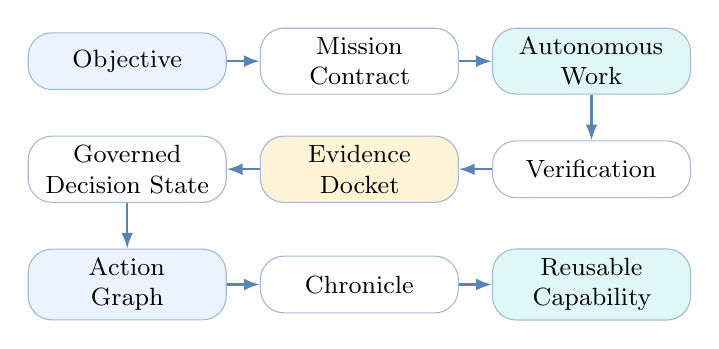
\begin{tikzpicture}[node distance=0.42cm, every node/.style={font=\small}, box/.style={rounded corners=3mm, draw=GoalBlue!42, fill=white, minimum height=0.72cm, align=center, text width=2.28cm}, arrow/.style={-{Latex[length=2mm]}, line width=0.8pt, color=GoalBlue!75}]
\node[box, fill=GoalSky] (o) {Objective};
\node[box, right=of o] (m) {Mission\\Contract};
\node[box, right=of m, fill=GoalCyan] (w) {Autonomous\\Work};
\node[box, below=0.58cm of w] (v) {Verification};
\node[box, left=of v, fill=GoalGoldLight] (d) {Evidence\\Docket};
\node[box, left=of d] (s) {Governed\\Decision State};
\node[box, below=0.58cm of s, fill=GoalSky] (a) {Action\\Graph};
\node[box, right=of a] (c) {Chronicle};
\node[box, right=of c, fill=GoalCyan] (r) {Reusable\\Capability};
\draw[arrow] (o)--(m); \draw[arrow] (m)--(w); \draw[arrow] (w)--(v); \draw[arrow] (v)--(d); \draw[arrow] (d)--(s); \draw[arrow] (s)--(a); \draw[arrow] (a)--(c); \draw[arrow] (c)--(r);
\end{tikzpicture}
\vfill
\begin{flushleft}
{\large Vincent Boucher}\par
{President, MONTREAL.AI and QUEBEC.AI}\par
\vspace{0.05in}
{\small June 2026. Written with AI. Publication-safe, claim-bounded edition.}\par
\end{flushleft}
\end{titlepage}

\begin{abstract}
\textbf{GoalOS Mission OS} is the commercial product layer for autonomous proof-to-action work. It turns a high-stakes objective into a \emph{Governed Decision State}: mission contract, claims matrix, source provenance, contradiction register, Evidence Docket, verifier report, risk ledger, executive brief, decision deck, action graph, Chronicle entry, and reusable capability package. This elevated edition adds the autonomous publication law: the public website is generated from proof-aligned source, checked by automation, opened as a human-review pull request, and published only after review. The claim is architectural and falsifiable. It does not claim achieved AGI, ASI, superintelligence, guaranteed returns, legal advice, financial advice, production certification, mainnet deployment, or civilization-scale capability. It defines a practical path for converting AI output into governed, auditable, reusable institutional capability.
\end{abstract}

\softlaw{A model can answer. An agent can act. An institution must prove. No proof, no settlement. No eval, no propagation. No rollback, no release.}

\tableofcontents
\newpage

\section{Executive thesis}
The first age of AI was the age of generation. Models made answers, drafts, code, reports, plans, and agent traces abundant. The next age is the age of proof. Institutions do not merely need more output; they need to know which output deserves trust, payment, propagation, reuse, and rollback authority.

GoalOS Mission OS is the operating layer between autonomous AI activity and institutional work. It does not compete by producing longer reports. It converts an objective into a governed decision state: evidence, verification, action, risk, memory, and reusable capability.

\begin{goldbox}
\textbf{Canonical product promise.} GoalOS Mission OS: The Proof OS for Autonomous AI Work. Set the objective. GoalOS runs until proof is done.
\end{goldbox}

The strategic distinction is compact:
\[
\text{Research assistant}=\text{topic}\rightarrow\text{report}.
\]
\[
\text{Mission OS}=\text{objective}\rightarrow\text{proof}\rightarrow\text{decision state}\rightarrow\text{action}\rightarrow\text{capability}.
\]

\section{Substrate lineage: from models to institutions}
The Transformer made intelligence scalable inside models. AGI ALPHA proposes the complementary substrate above models: agents, jobs, validators, tools, memory, incentives, markets, settlement, governance, capacity allocation, and strategic capability development. The objective is to convert model capability into verified machine labor, verified machine labor into reusable capability, and reusable capability into productive capacity.

GoalOS Mission OS makes that thesis operational at the product layer. A user does not need to understand the whole protocol. The user supplies an objective. GoalOS produces a mission contract, executes bounded work, packages evidence, checks claims, surfaces risks, and emits a decision state ready for review.

\section{Product definition}
\textbf{GoalOS Mission OS} is a proof-to-action operating system for autonomous AI work. It turns objectives into proof-backed mission packages.

\begin{longtable}{p{0.26\linewidth}p{0.66\linewidth}}
\toprule
\textbf{Component} & \textbf{Function} \\
\midrule
Mission Contract & Defines objective, decision to support, success criteria, failure criteria, constraints, allowed sources, risk class, output package, review requirement, and done condition. \\
Autonomous Mission Engine & Decomposes the objective into workstreams: research, source mapping, contradiction detection, risk analysis, action planning, verification, and packaging. \\
Verifier Mesh & Checks source reality, claim support, contradiction coverage, assumptions, freshness, risk, and claim boundaries. \\
Evidence Docket & Organizes evidence into a public-safe proof room with claims matrix, provenance, baselines, proof packets, risk/cost ledgers, and replay path. \\
Governed Decision State & Converts evidence into a decision package that can be inspected, defended, acted on, or rejected. \\
Action Graph & Converts recommendation into scoped next actions, dependencies, owners, approvals, proof requirements, and rollback conditions. \\
Chronicle & Records the mission, claims, evidence, decision state, action graph, and reusable capability package. \\
\bottomrule
\end{longtable}

\begin{bluebox}
\textbf{User-facing translation.} A normal person or organization does not ask GoalOS for more text. They ask GoalOS to move one objective from uncertainty to justified action.
\end{bluebox}

\section{The Governed Decision State}
The flagship deliverable is not a document. It is a governed decision state. A report is static; a governed decision state is inspectable, challengeable, and operational.

A Governed Decision State contains:
\begin{itemize}
\item objective and decision to support;
\item claims matrix and source provenance;
\item contradiction register and uncertainty ledger;
\item Evidence Docket and verifier report;
\item risk ledger and claim boundary;
\item executive brief and decision deck;
\item action graph and rollback/failure conditions;
\item Chronicle entry and capability package.
\end{itemize}

\keyline{The deliverable is not a document. The deliverable is a governed decision state.}

\section{Mission value equation}
GoalOS optimizes mission value, not report length:
\begin{equation}
\mathrm{MissionValue}=\frac{\mathrm{DecisionImpact}\times\mathrm{ProofIntegrity}\times\mathrm{Actionability}\times\mathrm{Reuse}}{\mathrm{Cost}+\mathrm{Risk}+\mathrm{Latency}+\mathrm{ProofDebt}}.
\end{equation}

The highest-value output is not the longest report. It is the shortest path from uncertainty to justified action.

Proof debt is the risk that unverified AI output becomes institutional default:
\begin{equation}
D_{proof}=\sum_i Impact_i\times Unverified_i\times Irreversibility_i\times Reuse_i.
\end{equation}

Mission OS reduces proof debt by making claims explicit, source-bound, risk-classed, and reviewable before action.

\section{The proof-to-action equation}
The general law of AI work is:
\begin{equation}
AIWork=Output\times Proof\times Validation\times Settlement\times Reuse.
\end{equation}
If proof is zero, institutional work is zero:
\begin{equation}
Proof=0 \Rightarrow TrustedWork=0.
\end{equation}

This converts autonomy from a marketing claim into a gated process. Autonomy runs until the evidence package is complete, not until a model sounds persuasive.

\section{Until-DONE autonomy}
Mission OS uses a run-to-completion state machine. It keeps advancing until every required artifact exists and every required gate passes.

\begin{center}
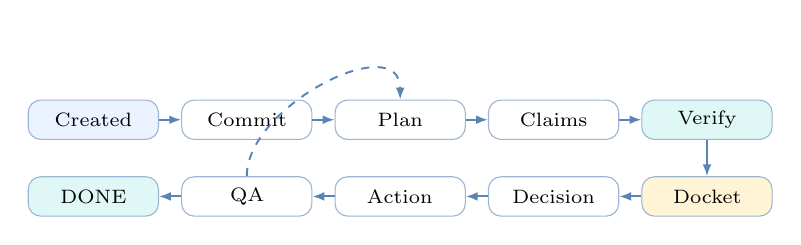
\begin{tikzpicture}[node distance=0.28cm, every node/.style={font=\scriptsize}, box/.style={rounded corners=1.6mm, draw=GoalBlue!45, fill=white, minimum height=0.50cm, align=center, text width=1.42cm}, arrow/.style={-{Latex[length=1.5mm]}, line width=0.7pt, color=GoalBlue!75}]
\node[box, fill=GoalSky] (a) {Created};
\node[box] (b) [right=of a] {Commit};
\node[box] (c) [right=of b] {Plan};
\node[box] (d) [right=of c] {Claims};
\node[box, fill=GoalCyan] (e) [right=of d] {Verify};
\node[box, fill=GoalGoldLight] (f) [below=0.46cm of e] {Docket};
\node[box] (g) [left=of f] {Decision};
\node[box] (h) [left=of g] {Action};
\node[box] (i) [left=of h] {QA};
\node[box, fill=GoalCyan] (j) [left=of i] {DONE};
\draw[arrow] (a)--(b); \draw[arrow] (b)--(c); \draw[arrow] (c)--(d); \draw[arrow] (d)--(e); \draw[arrow] (e)--(f); \draw[arrow] (f)--(g); \draw[arrow] (g)--(h); \draw[arrow] (h)--(i); \draw[arrow] (i)--(j);
\draw[arrow, dashed] (i.north) .. controls +(0,0.9) and +(0,0.9) .. (c.north);
\end{tikzpicture}
\end{center}

\begin{align}
DONE=1\Longleftrightarrow&\; MissionContract \land ClaimsMatrix \land SourceProvenance \\
&\land ContradictionRegister \land EvidenceDocket \land VerifierReport \\
&\land RiskLedger \land DecisionState \land ActionGraph \\
&\land ChronicleEntry \land ClaimBoundaryPass \land QAPass.
\end{align}

If a claim lacks evidence, the system returns to evidence gathering. If a contradiction is unresolved, it returns to analysis. If the risk ledger is missing, it returns to risk pass. If the claim boundary fails, it revises. If all gates pass, it emits a human-review-ready package.

\section{Evidence Docket and Verifier Mesh}
The Evidence Docket is the proof room. It is not a marketing page. It contains the claim, the supporting evidence, the baseline, the risk, the evaluator notes, the public-private boundary, and the replay or audit path.

\begin{center}
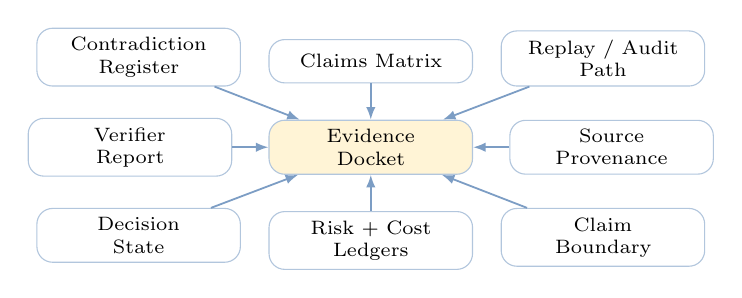
\begin{tikzpicture}[node distance=0.46cm, every node/.style={font=\scriptsize}, card/.style={rounded corners=2mm, draw=GoalBlue!35, fill=white, align=center, minimum height=0.55cm, text width=2.35cm}, arrow/.style={-{Latex[length=1.6mm]}, color=GoalBlue!60, line width=0.65pt}]
\node[card, fill=GoalGoldLight] (center) {Evidence\\Docket};
\node[card, above=of center] (claims) {Claims Matrix};
\node[card, right=of center] (prov) {Source\\Provenance};
\node[card, below=of center] (risk) {Risk + Cost\\Ledgers};
\node[card, left=of center] (verify) {Verifier\\Report};
\node[card, above left=0.42cm and 0.35cm of center] (contradict) {Contradiction\\Register};
\node[card, above right=0.42cm and 0.35cm of center] (replay) {Replay / Audit\\Path};
\node[card, below right=0.42cm and 0.35cm of center] (boundary) {Claim\\Boundary};
\node[card, below left=0.42cm and 0.35cm of center] (decision) {Decision\\State};
\foreach \n in {claims,prov,risk,verify,contradict,replay,boundary,decision}{\draw[arrow] (\n)--(center);}
\end{tikzpicture}
\end{center}

The Verifier Mesh asks a few simple but difficult questions: Are the sources real? Are primary and secondary sources separated? Are the claims supported? Are contradictions surfaced? Are assumptions explicit? Are time-sensitive facts dated? Are recommendations traceable to evidence? Are risks visible? Are unsafe claims blocked?

\section{Autonomous website publication law}
The website should not be hand-edited as a fragile public artifact. It should be generated from proof-aligned source, checked by automation, reviewed by a human, and then published. This is the same constitutional pattern applied to communication.

\begin{goldbox}
\textbf{Publication law.} The website is not hand-edited. It is generated from proof-aligned source, checked by automation, reviewed by a human, and then published.
\end{goldbox}

The autonomous publication pipeline is:
\[
ContentSource \rightarrow Generator \rightarrow QA \rightarrow PullRequest \rightarrow HumanReview \rightarrow Publish.
\]

\begin{center}
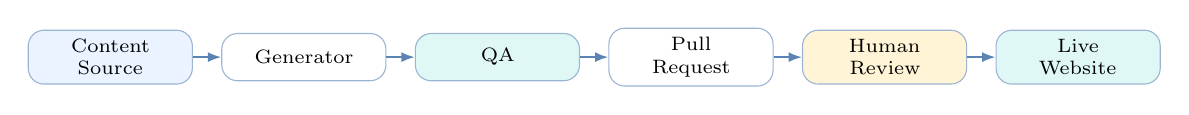
\begin{tikzpicture}[node distance=0.36cm, every node/.style={font=\scriptsize}, box/.style={rounded corners=2mm, draw=GoalBlue!45, fill=white, minimum height=0.60cm, align=center, text width=1.85cm}, arrow/.style={-{Latex[length=1.7mm]}, line width=0.72pt, color=GoalBlue!75}]
\node[box, fill=GoalSky] (source) {Content\\Source};
\node[box] (gen) [right=of source] {Generator};
\node[box, fill=GoalCyan] (qa) [right=of gen] {QA};
\node[box] (pr) [right=of qa] {Pull\\Request};
\node[box, fill=GoalGoldLight] (human) [right=of pr] {Human\\Review};
\node[box, fill=GoalCyan] (live) [right=of human] {Live\\Website};
\draw[arrow] (source)--(gen); \draw[arrow] (gen)--(qa); \draw[arrow] (qa)--(pr); \draw[arrow] (pr)--(human); \draw[arrow] (human)--(live);
\end{tikzpicture}
\end{center}

The workflow must not auto-merge, move tokens, broadcast mainnet transactions, publish unsupported claims, or remove claim boundaries. It may generate pages, reports, status files, and pull requests.

\section{Main website completeness standard}
The main website should behave as the institutional front door. It should be complete, clear, current, beautiful, useful, and safe. The Mission OS page should not be an isolated landing page; it should connect to Start, Autopilot, Use Cases, Proof Cards, Resources, Evidence Dockets, and the GitHub implementation.

Minimum standard:
\begin{itemize}
\item every page has a clear user path and no blank-rendering states;
\item important pages are generated from source or explicitly marked as hand-authored;
\item links to Mission OS, Autopilot, Use Cases, Proof Cards, and Resources stay live;
\item public claims include visible claim boundaries;
\item pages explain what normal users can do next;
\item diagrams are illustrated, legible, and not dependent on external asset loading;
\item automation opens human-review PRs rather than silently changing public pages.
\end{itemize}

\section{Commercial wedge: proof missions}
The immediate commercial product is a 48-hour proof mission.

\begin{plaincard}
\textbf{Founding offer.} Give GoalOS one high-stakes objective. Receive a proof-backed governed decision state: Evidence Docket, verifier report, risk ledger, executive brief, decision deck, action graph, Chronicle entry, and capability package.
\end{plaincard}

Best initial use cases include AI product intelligence, enterprise AI adoption, market entry, policy and regulation options, competitive strategy, procurement review, partnership diligence, and defensive cybersecurity readiness. The strongest proof mission is not the largest report. It is the one that makes a decision inspectable, defensible, and actionable.

\section{Conformance levels}
Mission OS can be adopted incrementally.

\begin{longtable}{p{0.12\linewidth}p{0.23\linewidth}p{0.55\linewidth}}
\toprule
\textbf{Level} & \textbf{Name} & \textbf{Requirement} \\
\midrule
L0 & Source-valid & Content source, mission schema, and generator inputs validate. \\
L1 & Page-generating & The page or mission package is generated deterministically from source. \\
L2 & QA-gated & Automation checks links, required sections, claim boundary, and blank-render prevention. \\
L3 & Evidence-emitting & Mission run emits Evidence Docket, verifier report, risk ledger, action graph, and run state. \\
L4 & Human-reviewed & Generated changes are opened as a pull request and require human review. \\
L5 & Chronicle-ready & Accepted outputs write Chronicle entries and capability packages. \\
L6 & Cross-institutional & Proof-carrying artifacts can be reused across organizations without exposing private intelligence. \\
\bottomrule
\end{longtable}

\section{Safety and claim boundary}
The architecture is deliberately claim-bounded. Mission OS does not claim achieved AGI, achieved ASI, superintelligence, external audit completion, production certification, guaranteed ROI, legal advice, financial advice, medical advice, public benchmark SOTA, mainnet deployment, autonomous sovereignty, energy abundance, or civilization-scale capability.

\begin{boundarybox}
\textbf{Claim boundary.} GoalOS Mission OS is a proof-to-action architecture, implementation, and publication system. It becomes empirical only through real tasks, evidence dockets, baselines, replay, cost/risk ledgers, verifier reports, delayed outcomes, and independent review.
\end{boundarybox}

\section{Evaluation program}
The evaluation program tests whether Mission OS outperforms report-only baselines and ad-hoc agent workflows.

\begin{longtable}{p{0.30\linewidth}p{0.62\linewidth}}
\toprule
\textbf{Evaluation} & \textbf{What must be measured} \\
\midrule
Report baseline & Does Mission OS produce more actionable, evidence-bound, and reviewable output than a report-only system? \\
Claim support & What share of major claims are linked to sources or explicit uncertainty? \\
Contradiction handling & Are conflicting sources or assumptions surfaced rather than hidden? \\
Decision readiness & Can a reviewer understand options, risks, and next actions without reading all raw traces? \\
Proof debt reduction & Does the mission reduce unsupported assumptions and unreviewed AI output? \\
Reuse & Does the capability package improve future related missions? \\
Safety & Are unsupported claims, sensitive data leakage, and unsafe actions blocked? \\
Publication QA & Does the generated website remain visible, complete, accessible, and claim-bounded? \\
\bottomrule
\end{longtable}

\section{Implementation path}
The current practical path is:
\begin{enumerate}
\item Upload the autonomous website source, generator, docs, and workflows.
\item Run the website autopilot workflow in generate-PR mode.
\item Review the PR for visible page quality and claim boundary.
\item Merge only after the generated status and report pass.
\item Run the Mission OS until-DONE workflow on a public-safe example mission.
\item Publish the first Evidence Docket and governed decision state.
\item Open founding proof mission slots.
\end{enumerate}

\section{Conclusion}
GoalOS Mission OS gives GoalOS a concrete commercial front end. It is not merely a research assistant, an agent swarm, or a report generator. It is a proof-to-action operating system for autonomous AI work.

The public thesis is short:
\begin{goldbox}
\textbf{GoalOS Mission OS.} Set the objective. GoalOS runs until proof is done. AI creates output. GoalOS creates proof. The deliverable is a governed decision state.
\end{goldbox}

The institutional law is stricter:
\begin{mintbox}
No proof, no settlement. No eval, no propagation. No rollback, no release.
\end{mintbox}

The next proof is not another claim. It is a public-safe mission run that reaches DONE=true and publishes an Evidence Docket people can inspect.

\section*{References}
\begin{enumerate}[label={[\arabic*]}, leftmargin=1.8em]
\item Vincent Boucher. \emph{AGI ALPHA: A Scalable Substrate for Intelligence Organizations}. 2026. Used for organizational-substrate lineage, Evidence Docket discipline, ProofBundles, replay logs, cost/safety ledgers, validators, and governed recursive improvement.
\item Vincent Boucher. \emph{GoalOS: The Proof-of-Evolution Constitution, AEP-001}. 2026. Used for the public/private proof boundary, proof-carrying artifacts, Proof Gradient, Evolution Ledger, Evidence Docket, and constitutional doctrine.
\item Supplied frontier-verifiability context. Used only as strategic context for the importance of verifiable signal, reward soundness, and long-horizon proof-bearing work. Public GoalOS language remains independent and GoalOS-native.
\item Supplied startup-growth context. Used only as product strategy context: users share products that create value they care about; GoalOS should make proof-backed progress worth sharing.
\end{enumerate}

\end{document}
